\documentclass{beamer}\usepackage[]{graphicx}\usepackage[]{xcolor}
% maxwidth is the original width if it is less than linewidth
% otherwise use linewidth (to make sure the graphics do not exceed the margin)
\makeatletter
\def\maxwidth{ %
  \ifdim\Gin@nat@width>\linewidth
    \linewidth
  \else
    \Gin@nat@width
  \fi
}
\makeatother

\definecolor{fgcolor}{rgb}{0.345, 0.345, 0.345}
\newcommand{\hlnum}[1]{\textcolor[rgb]{0.686,0.059,0.569}{#1}}%
\newcommand{\hlstr}[1]{\textcolor[rgb]{0.192,0.494,0.8}{#1}}%
\newcommand{\hlcom}[1]{\textcolor[rgb]{0.678,0.584,0.686}{\textit{#1}}}%
\newcommand{\hlopt}[1]{\textcolor[rgb]{0,0,0}{#1}}%
\newcommand{\hlstd}[1]{\textcolor[rgb]{0.345,0.345,0.345}{#1}}%
\newcommand{\hlkwa}[1]{\textcolor[rgb]{0.161,0.373,0.58}{\textbf{#1}}}%
\newcommand{\hlkwb}[1]{\textcolor[rgb]{0.69,0.353,0.396}{#1}}%
\newcommand{\hlkwc}[1]{\textcolor[rgb]{0.333,0.667,0.333}{#1}}%
\newcommand{\hlkwd}[1]{\textcolor[rgb]{0.737,0.353,0.396}{\textbf{#1}}}%
\let\hlipl\hlkwb

\usepackage{framed}
\makeatletter
\newenvironment{kframe}{%
 \def\at@end@of@kframe{}%
 \ifinner\ifhmode%
  \def\at@end@of@kframe{\end{minipage}}%
  \begin{minipage}{\columnwidth}%
 \fi\fi%
 \def\FrameCommand##1{\hskip\@totalleftmargin \hskip-\fboxsep
 \colorbox{shadecolor}{##1}\hskip-\fboxsep
     % There is no \\@totalrightmargin, so:
     \hskip-\linewidth \hskip-\@totalleftmargin \hskip\columnwidth}%
 \MakeFramed {\advance\hsize-\width
   \@totalleftmargin\z@ \linewidth\hsize
   \@setminipage}}%
 {\par\unskip\endMakeFramed%
 \at@end@of@kframe}
\makeatother

\definecolor{shadecolor}{rgb}{.97, .97, .97}
\definecolor{messagecolor}{rgb}{0, 0, 0}
\definecolor{warningcolor}{rgb}{1, 0, 1}
\definecolor{errorcolor}{rgb}{1, 0, 0}
\newenvironment{knitrout}{}{} % an empty environment to be redefined in TeX

\usepackage{alltt}
\mode<presentation>
{
  \usetheme{default}                    % Set theme
  \usecolortheme{default}               % Set colors
  \usefonttheme{default}                % Set font theme
  \setbeamertemplate{caption}[numbered] % Set caption to be numbered
}
\usepackage{lipsum}
\usepackage{graphicx}  % For including figures
\usepackage{booktabs}  % For table rules
\usepackage{hyperref}
\usepackage{siunitx}
\title{Exploratory Analysis of a Crime Data}  % Presentation title
\author{Team: Extra-Idiotic Family}                              % Presentation author
\institute{University of Nebraska-Lincoln}                  % Author affiliation
\date{\today}
\IfFileExists{upquote.sty}{\usepackage{upquote}}{}
\begin{document}

\begin{frame}
  \titlepage
\end{frame}

\begin{frame}{Dataset Discription}

This dataset reflects incidents of crime in the City of Los Angeles dating back to 2020. There are 521k rows (each row is a crime incident) and 28 columns (Variables)

Data set link: \href{https://data.lacity.org/Public-Safety/Crime-Data-from-2020-to-Present/2nrs-mtv8}{here}.



\begin{knitrout}
\definecolor{shadecolor}{rgb}{0.969, 0.969, 0.969}\color{fgcolor}
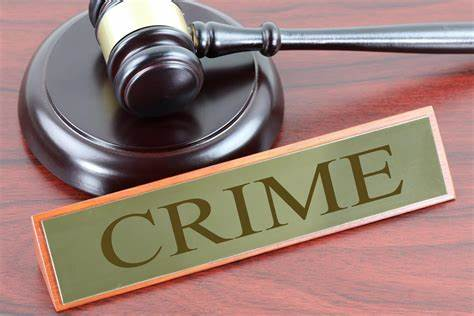
\includegraphics[width=0.5\textwidth]{figure/title.jpg}
\end{knitrout}
\end{frame}

\begin{frame}{Variables Used under Analysis}

\begin{itemize}
\item Initially there were 28 variables in the data set.
\item We focused only several variables for our analysis.
\end{itemize}



\begin{tabular}{|c||c|}
\hline
    Variable & Description \\ 
\hline
    AREA & Geographic Areas in Los-Angeles \\ 
\hline
    AREA NAME & Name designation of the area \\ 
\hline
Crm cd & crime code\\
\hline
Crm cd Desc & Defines the crime Code Provided\\
\hline
Vict Age & Age of the Victim\\
\hline
Vict Sex & Sex of the Victim\\
\hline
Vict Descent & Descent Code of the Victim\\
\hline
Premis Desc & Premises Description\\
\hline
Weapon Desc & weapon used in crime\\
\hline
\end{tabular}
\end{frame}

\begin{frame}[fragile]{Method and analysis (re-categorizing crimes)}
\begin{itemize}
\item originally there were 73 types of crime.
\item We re-categorized them as follows
\end{itemize}

\begin{knitrout}
\definecolor{shadecolor}{rgb}{0.969, 0.969, 0.969}\color{fgcolor}
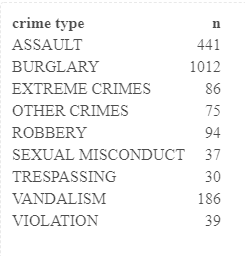
\includegraphics[width=\maxwidth]{figure/crime_types.png} 
\end{knitrout}

\end{frame}

\begin{frame}[fragile]{Method and analysis (Cleaning Age variable)}
\begin{columns}
		\column{.6\textwidth}
\begin{knitrout}
\definecolor{shadecolor}{rgb}{0.969, 0.969, 0.969}\color{fgcolor}
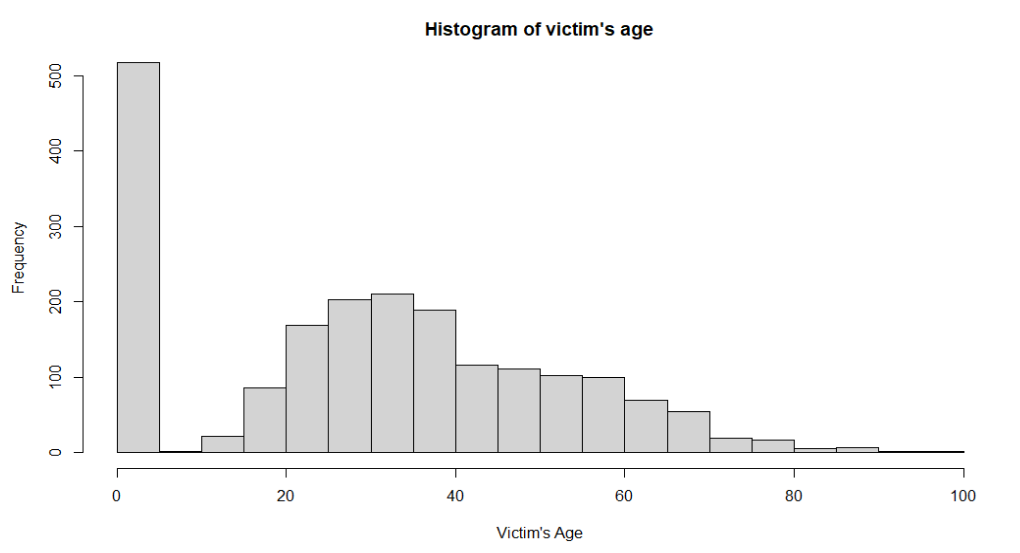
\includegraphics[width=\maxwidth]{figure/hist_age.png} 
\end{knitrout}

\column{.4\textwidth}
\textbf{Highlights}
\begin{itemize}
\item Unusual number of Zero records.
\item replace them with median of age. 
\item continue the analysis.

\end{itemize}

\end{columns}
\end{frame}

\begin{frame}[fragile]{Method and analysis (Re-categorizing Descent variable)}
\begin{columns}
		\column{.5\textwidth}
\begin{knitrout}
\definecolor{shadecolor}{rgb}{0.969, 0.969, 0.969}\color{fgcolor}
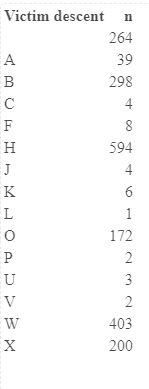
\includegraphics[width=\maxwidth]{figure/Des_categories.png} 
\end{knitrout}

\column{.5\textwidth}
\begin{tabular}{|c||c|}
\hline
    Symbol & Descecnt \\ 
\hline
    A & Other Asian \\ 
\hline
    B & Black \\ 
\hline
H & Hispanic/Latin/Mexican\\
\hline
O & other\\
\hline
W & white\\
\hline
 & Minor or Unknown\\
\hline

\end{tabular}

\end{columns}
\end{frame}

\begin{frame}[fragile]{relationship with the area and the crime}

which area is the most awfull to live.

\begin{knitrout}
\definecolor{shadecolor}{rgb}{0.969, 0.969, 0.969}\color{fgcolor}
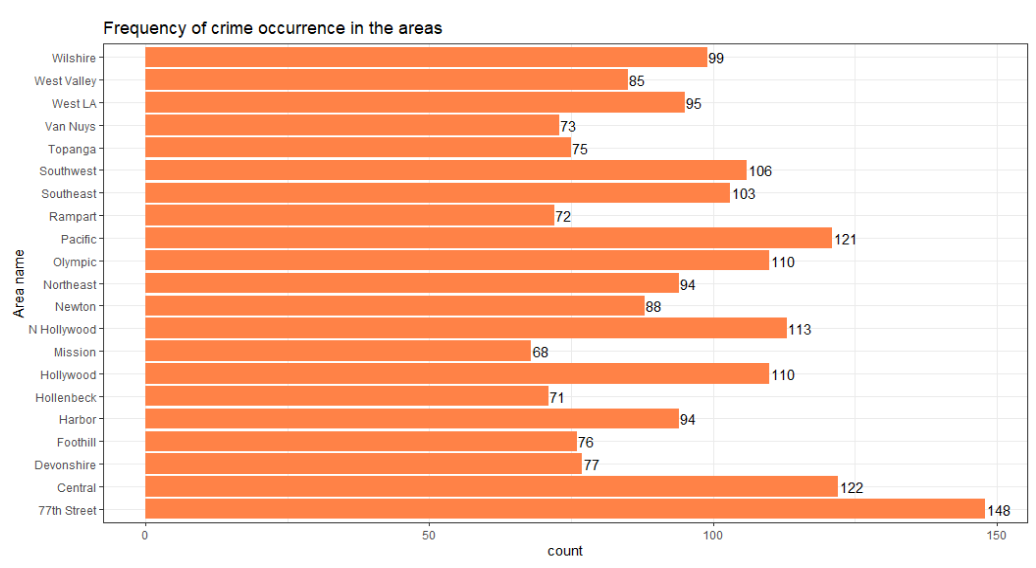
\includegraphics[width=\maxwidth]{figure/place.png} 
\end{knitrout}
\textbf{Highlights}
\begin{itemize}
\item 77th street has the highest number of crimes.
\item 100+ crimes have been reported over some other areas
\item Please avoid those areas.

\end{itemize}
\end{frame}

\begin{frame}[fragile]{Which type of crimes ocured most}
\begin{columns}
		\column{.5\textwidth}
\begin{knitrout}
\definecolor{shadecolor}{rgb}{0.969, 0.969, 0.969}\color{fgcolor}
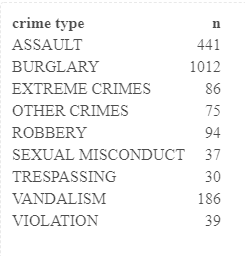
\includegraphics[width=\maxwidth]{figure/crime_types.png} 
\end{knitrout}

\column{.5\textwidth}
\textbf{Highlights}
\begin{itemize}
\item Burglary And Assault
\begin{knitrout}
\definecolor{shadecolor}{rgb}{0.969, 0.969, 0.969}\color{fgcolor}
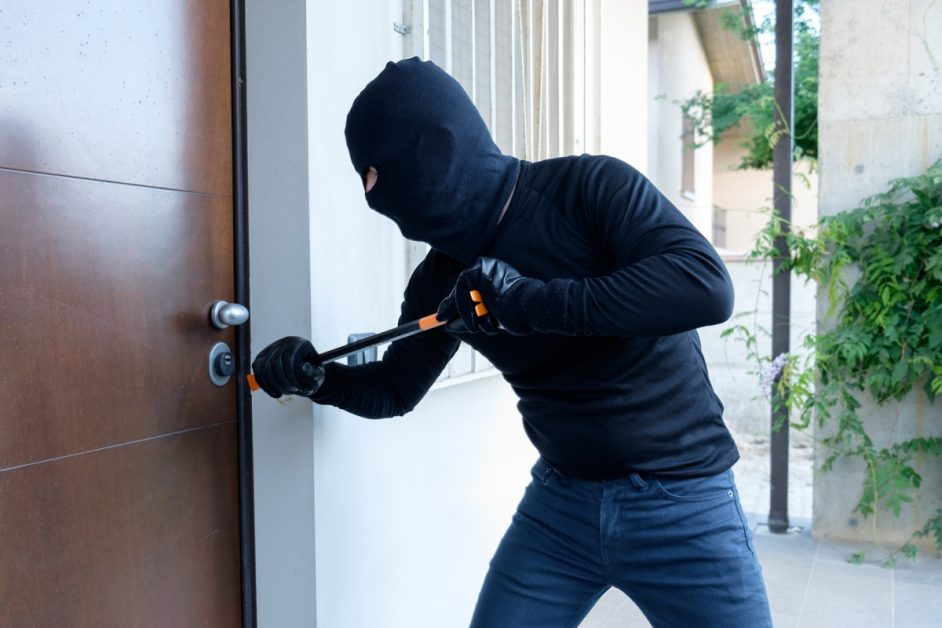
\includegraphics[width=\maxwidth]{figure/bur.jpg} 
\end{knitrout}
\begin{knitrout}
\definecolor{shadecolor}{rgb}{0.969, 0.969, 0.969}\color{fgcolor}
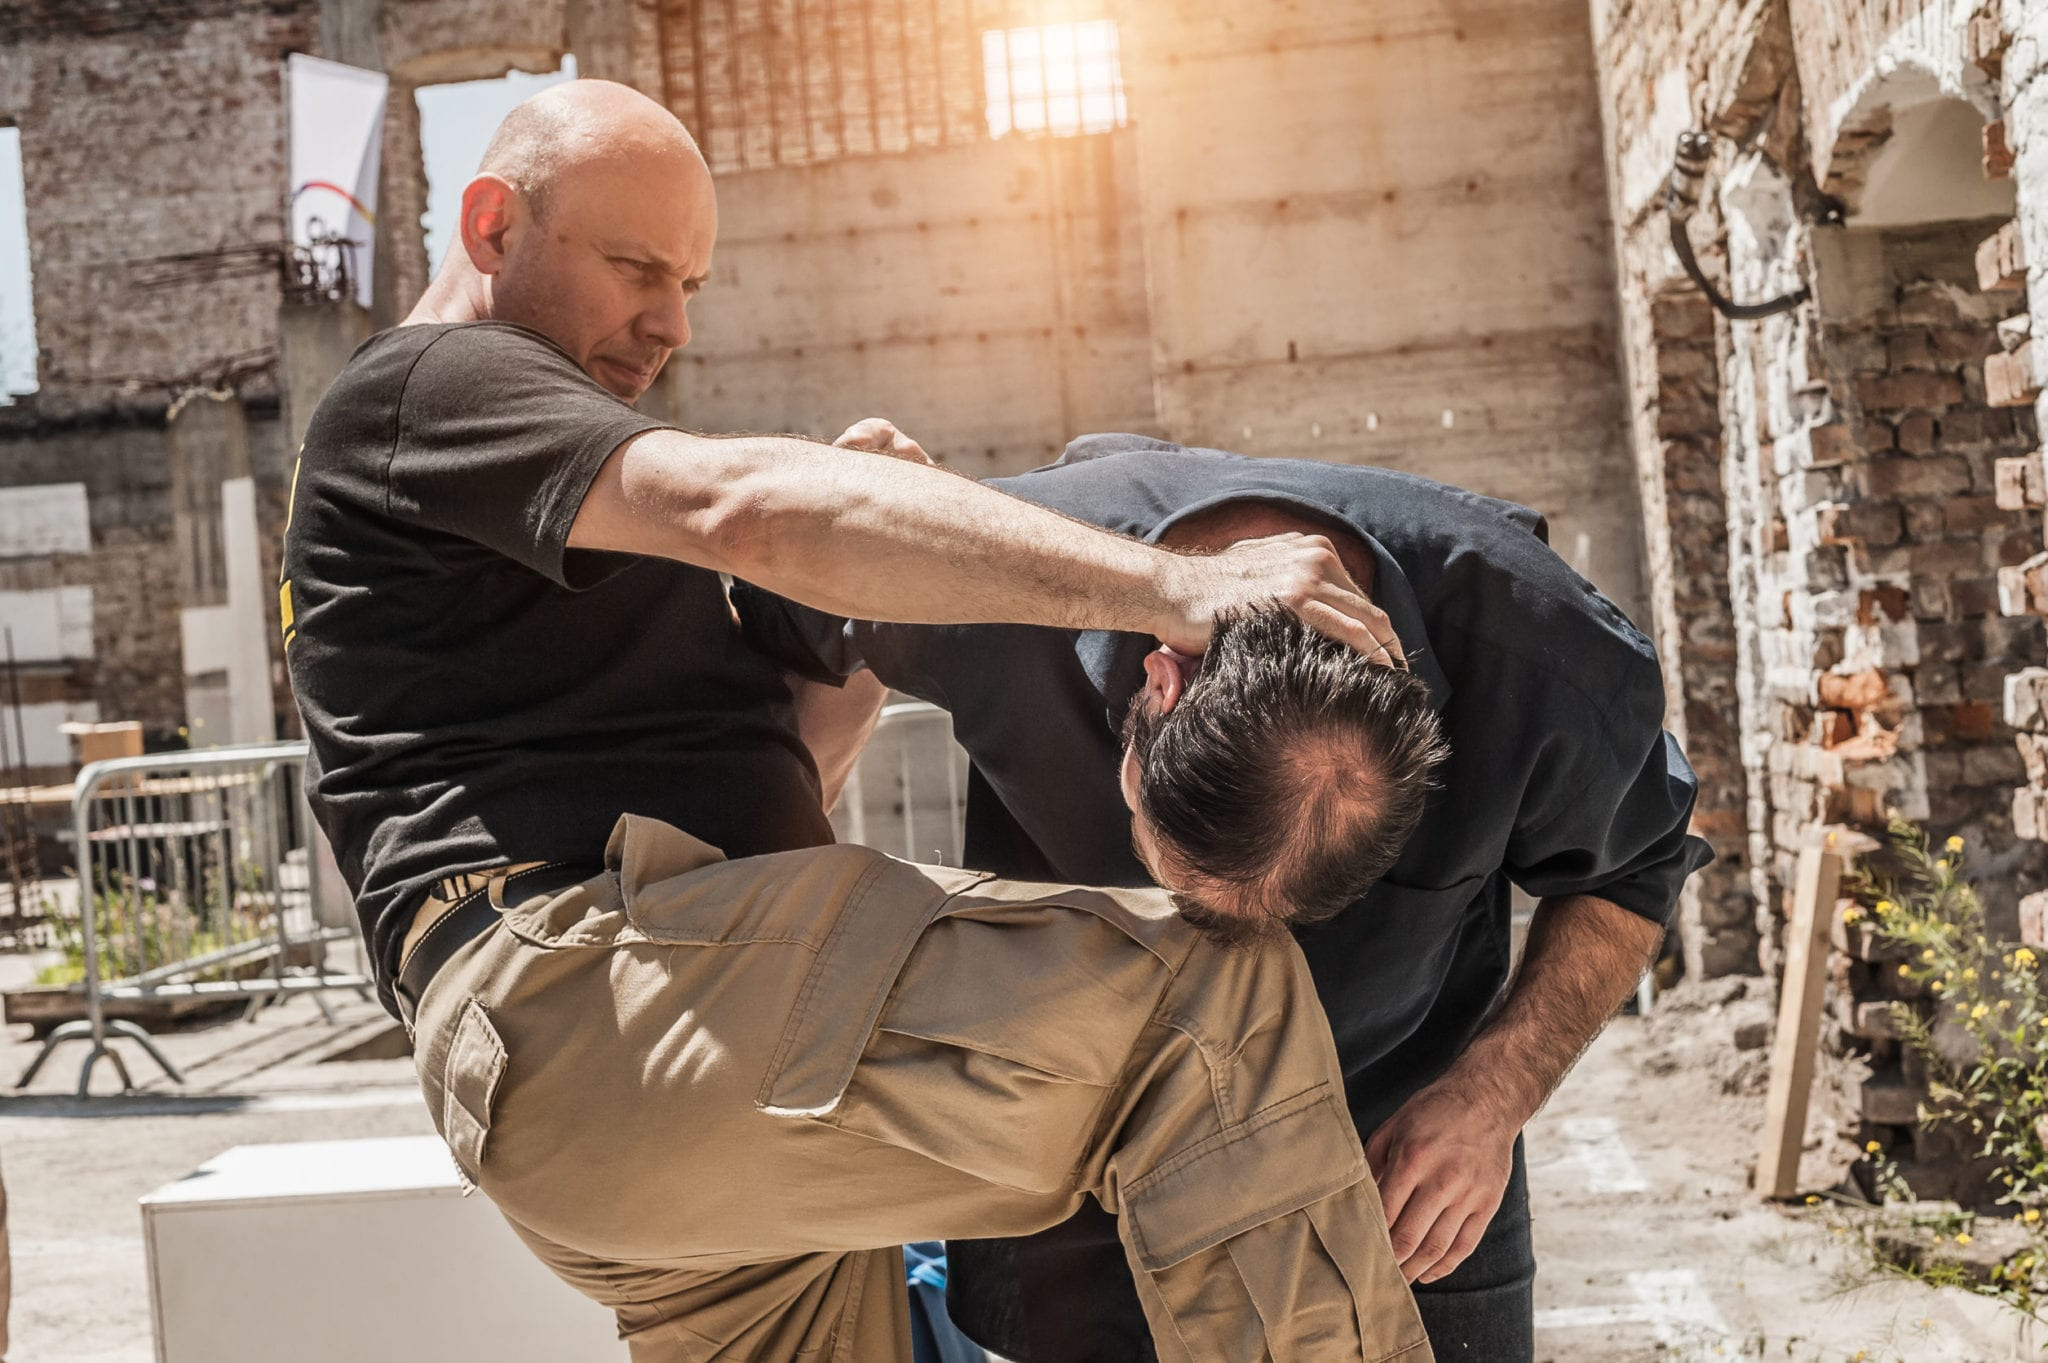
\includegraphics[width=\maxwidth]{figure/as.jpg} 
\end{knitrout}
\end{itemize}

\end{columns}
\end{frame}

\begin{frame}[fragile]{Relationship between the area and the crime "Assault"}

\begin{knitrout}
\definecolor{shadecolor}{rgb}{0.969, 0.969, 0.969}\color{fgcolor}
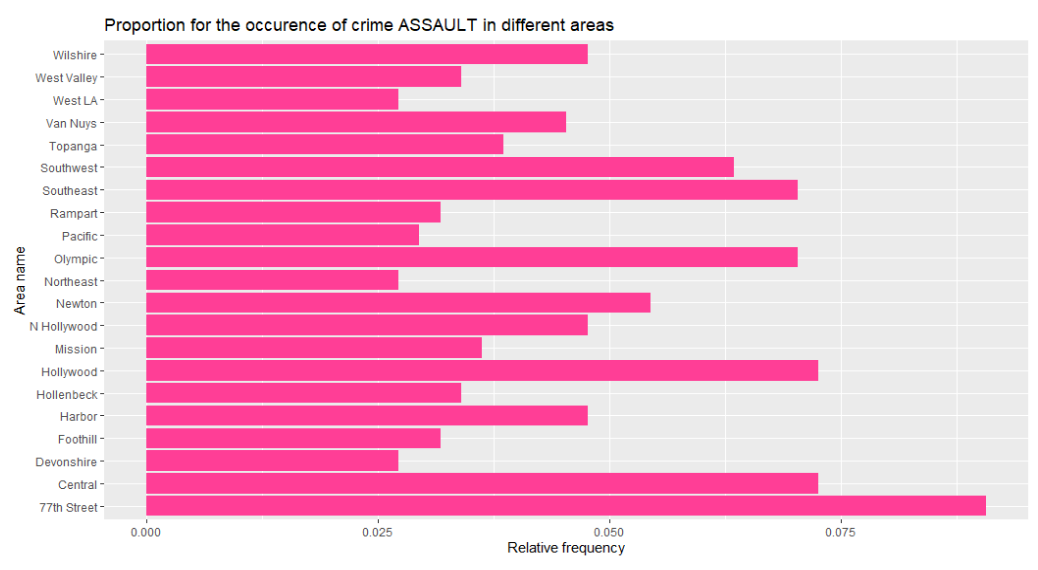
\includegraphics[width=\maxwidth]{figure/assault.png} 
\end{knitrout}
\textbf{Highlights}
\begin{itemize}
\item 77th street 
\item Southeast, Olymic, Hollywood, Central

\end{itemize}
\end{frame}

\begin{frame}[fragile]{Relationship between the area and the crime "Burglary"}

\begin{knitrout}
\definecolor{shadecolor}{rgb}{0.969, 0.969, 0.969}\color{fgcolor}
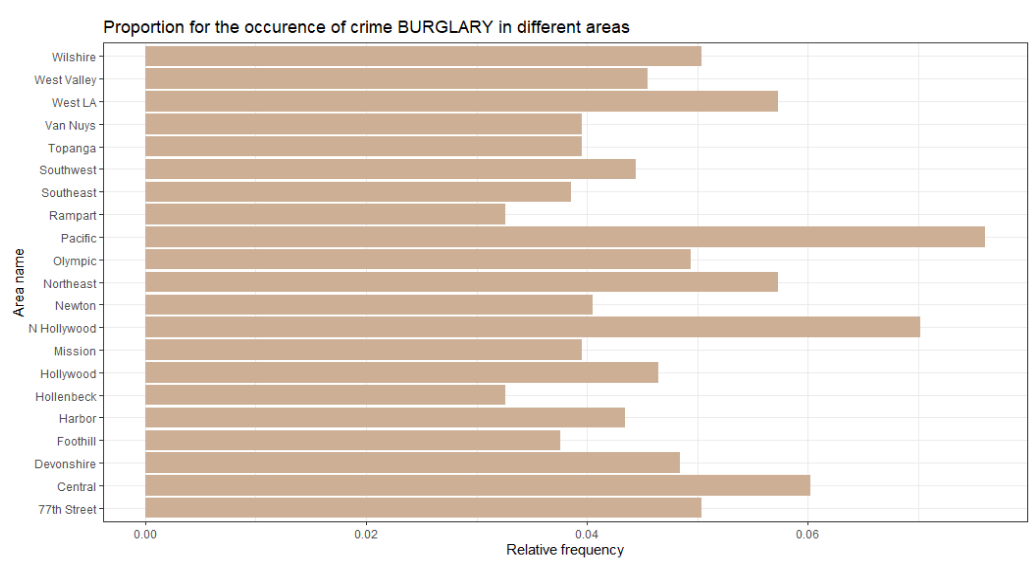
\includegraphics[width=\maxwidth]{figure/burglary.png} 
\end{knitrout}
\textbf{Highlights}
\begin{itemize}
\item Pacific 
\item West LA, Northeast, N Hollywood, Central

\end{itemize}
\end{frame}

\begin{frame}[fragile]{Relationship between the age and the crime type}

\begin{knitrout}
\definecolor{shadecolor}{rgb}{0.969, 0.969, 0.969}\color{fgcolor}
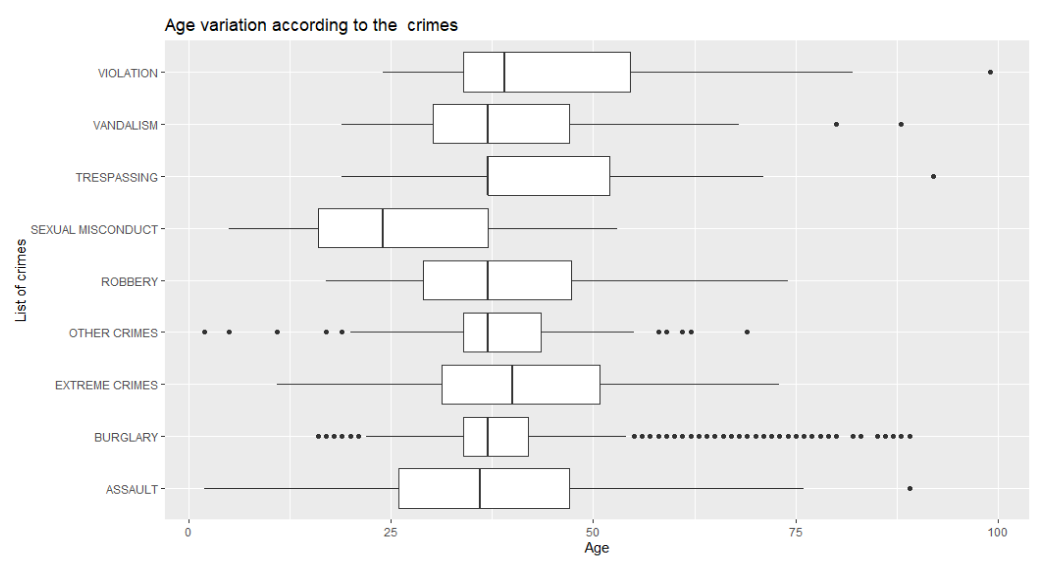
\includegraphics[width=\maxwidth]{figure/box_age.png} 
\end{knitrout}
\textbf{Highlights}
\begin{itemize}
\item Sexual Misconduct

\end{itemize}
\end{frame}

\begin{frame}[fragile]{Relationship between the Descent and the crime type}

\begin{knitrout}
\definecolor{shadecolor}{rgb}{0.969, 0.969, 0.969}\color{fgcolor}
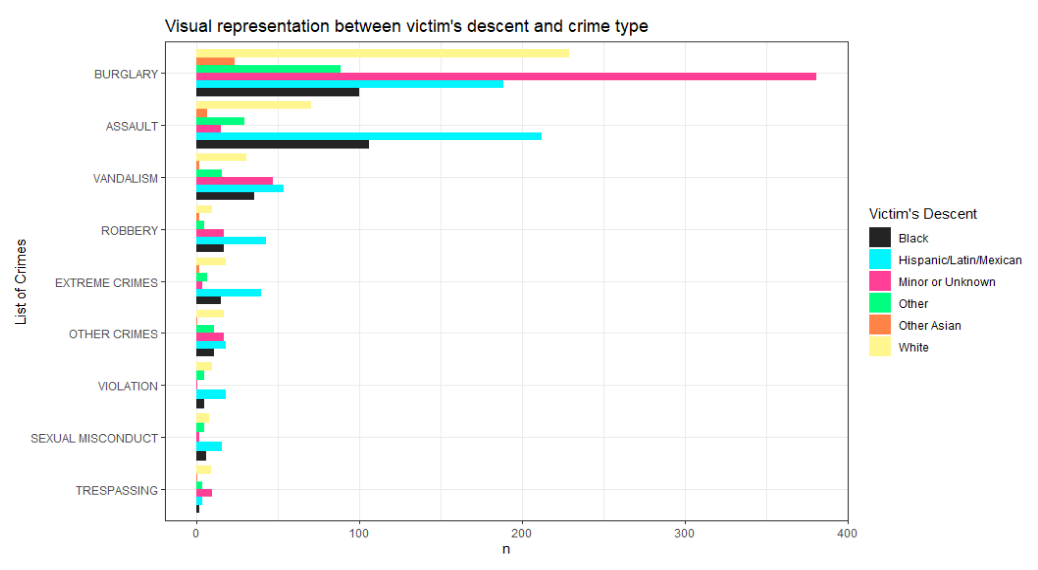
\includegraphics[width=\maxwidth]{figure/descent.png} 
\end{knitrout}
\textbf{Highlights}
\begin{itemize}
\item Burglary -> White people
\item All other types -> Hispanic/Latin/Mexican people
\end{itemize}
\end{frame}

\end{document}
